
\documentclass[sigconf]{acmart}

%%
%% \BibTeX command to typeset BibTeX logo in the docs
\AtBeginDocument{%
  \providecommand\BibTeX{{%
    \normalfont B\kern-0.5em{\scshape i\kern-0.25em b}\kern-0.8em\TeX}}}

%% Rights management information.  This information is sent to you
%% when you complete the rights form.  These commands have SAMPLE
%% values in them; it is your responsibility as an author to replace
%% the commands and values with those provided to you when you
%% complete the rights form.
\setcopyright{acmcopyright}
\copyrightyear{2019}
\acmYear{2019}
%%\acmDOI{}

\settopmatter{printacmref=false}

%% These commands are for a PROCEEDINGS abstract or paper.
\acmConference[ACSAC '19]{ACSAC '19: }{Dec. 09--13, 2019}{San Juan, Puerto Rico}
%%\acmBooktitle{ACSCAC '19: Annual Computer Security Applications Conference Dec. 09--13, 2019, San Juan, Puerto Rico}
%%\acmPrice{15.00}
%%\acmISBN{978-1-4503-9999-9/18/06}

\usepackage{algorithm}
\usepackage{algorithmic}
\usepackage{pgfplots}
\usepackage{tikz}
\usetikzlibrary{shapes,arrows}
\usepackage{flushend}

\usepackage[title]{appendix}

%%
%% Submission ID.
%% Use this when submitting an article to a sponsored event. You'll
%% receive a unique submission ID from the organizers
%% of the event, and this ID should be used as the parameter to this command.
%%\acmSubmissionID{123-A56-BU3}

%%
%% The majority of ACM publications use numbered citations and
%% references.  The command ~\citestyle{authoryear} switches to the
%% "author year" style.
%%~\citestyle{acmauthoryear}

%%
%% end of the preamble, start of the body of the document source.
\begin{document}

%%
%% The "title" command has an optional parameter,
%% allowing the author to define a "short title" to be used in page headers.
\title{All Jelly No Jam}
\subtitle{Mitigating Interleaving Targeted Jamming of IEEE802.11}

%%
%% The "author" command and its associated commands are used to define
%% the authors and their affiliations.
%% Of note is the shared affiliation of the first two authors, and the
%% "authornote" and "authornotemark" commands
%% used to denote shared contribution to the research.
\author{Benjamin Davis}
\email{bdavis41@calpoly.edu}
%%\orcid{1234-5678-9012}
\affiliation{%
  \institution{California Polytechnic State University}
  \city{San Luis Obispo}
  \state{California}
}

\author{Bruce DeBruhl}
\email{bdebruhl@calpoly.edu}
%%\orcid{1234-5678-9012}
\affiliation{%
  \institution{California Polytechnic State University}
  \city{San Luis Obispo}
  \state{California}
}


\renewcommand{\shortauthors}{Davis and DeBruhl}

%%
%% The abstract is a short summary of the work to be presented in the
%% article.
\begin{abstract}
  Recent jamming attacks against OFDM based IEEE 802.11 (WiFi) have targeted the interleaving mechanism to greatly improve the power efficiency of such attacks, getting as good as 95\% packet loss at 0.1\% power of the transmitter. This paper proposes a novel method of modifying the interleaver to prevent this attack vector through using a shared secret to deterministically interleave the data in such a way that is not susceptible to targeted sub-carrier jamming. We implement and test this approach using software defined radio. We show it entirely negates the impact of interleaving targeted jamming, without making the signal more susceptible to more traditional jamming methods or additive white Gaussian noise. We show that our modified interleaver makes these attacks less effective than whole-channel jamming by as much as 15\% lower packet loss.
\end{abstract}

%%
%% The code below is generated by the tool at http://dl.acm.org/ccs.cfm.
%% Please copy and paste the code instead of the example below.
%%
\begin{CCSXML}
<ccs2012>
<concept>
<concept_id>10002978.10003014.10003017</concept_id>
<concept_desc>Security and privacy~Mobile and wireless security</concept_desc>
<concept_significance>500</concept_significance>
</concept>
<concept>
<concept_id>10002978.10003006.10011610</concept_id>
<concept_desc>Security and privacy~Denial-of-service attacks</concept_desc>
<concept_significance>300</concept_significance>
</concept>
<concept>
<concept_id>10003033.10003083.10003095</concept_id>
<concept_desc>Networks~Network reliability</concept_desc>
<concept_significance>100</concept_significance>
</concept>
</ccs2012>
\end{CCSXML}

\ccsdesc[500]{Security and privacy~Mobile and wireless security}
\ccsdesc[300]{Security and privacy~Denial-of-service attacks}
\ccsdesc[100]{Networks~Network reliability}

%%
%% Keywords. The author(s) should pick words that accurately describe
%% the work being presented. Separate the keywords with commas.
\keywords{WiFi, Jamming, Interleaver}

%%
%% This command processes the author and affiliation and title
%% information and builds the first part of the formatted document.
\maketitle

\section{Introduction}

Wireless communication technology is ubiquitous in a wide variety of modern consumer applications. What at one point was nearly explicitly used for the transmission of data for defense applications has fully permeated into civilian day-to-day life. Technologies such as GPS, cellular data, and WiFi have become so common that many people could not imagine life without them. However, the very nature of wireless data transfer exposes them to host of vulnerabilities not practical in wired transmission. Chief concerns among these are data leakage, data spoofing, and denial-of-service (DoS) attacks. DoS attacks are particularly concerning because they are able to bring an entire data channel down with minimal effort. In the early 2010's a series of cellular and GPS jamming attacks in the wild prompted the FCC to further its own education and enforcement efforts against jammers~\cite{FCC2011enforcement}. Some companies have even been fined when it was determined they were deliberately jamming particular wireless networks~\cite{FCC2014marriott}.  In the previous example, we note that commodity consumer devices were targeted.  

Recently, jamming attacks against IEEE 802.11 (WiFi) have been a prominent area of research. This is likely because of the ubiquity and prevalence of WiFi in a connected world. Among these are attacks which target the preamble~\cite{mueller2013efficient, la2013phase} of WiFi and the Pilot channels~\cite{clancy2011efficient} to strong effect. Recently, Vo-Huu et al. published an attack paper which describes highly efficient jamming using the static nature of the interleaving mechanism of 802.11 to achieve 95\% packet loss at 0.1\% of the transmitter power (see Section~\ref{sec:jamming})~\cite{vo2016interleaving}. Interleaving addresses two problems of RF data transfer: bursty errors and channel bias. Bursty error occur when noise naturally manifests itself across a frequency and forces the data on that frequency to become invalid. Channel bias occurs through some mediums and in some environments where a RF signal might be naturally forced towards a specific value. This can in turn cause a sufficient number of bit errors to overwhelm any error correction coding.

In their paper, Vo-Huu et al. show that they are able to obtain 100\% packet error rate with a signal-to-jamming ratio of only 1\%. This attack is particularly concerning because it can be easily implemented on inexpensive hardware at a high power to impact a wide area. Additionally, while the attack is conducted on WiFi it is not the only wireless data transfer protocol with a static interleaver meaning there are other systems which are vulnerable to this attack vector as well. Notable examples being LoRa and GSM Voice's use of a diagonal interleaver as data-link being employed in military applications~\cite{knight2016decoding}. Although there already exist a variety of anti-jamming techniques for use in modern RF data transfer, to the best of our knowledge, none of these were designed with interleaver jamming in mind and many of them appear to be susceptible to interleaving targeted jamming. 

In this paper we propose and test Jelly interleaving, a novel interleaving mechanism designed to mitigate the impact of interleaving jamming without negatively impacting speed or noise resistance. In our protocol, we seek to establish a shared secret and use it to construct an interleaving mechanism which distributes adjacent bits in a non-predictable pattern. Through testing we are able to show that our modifications completely negate this particular jamming attack, in fact reducing its effect so this attack is less power efficient than whole-channel jamming by 15\%.

The remainder of the paper is structured as follows. In Section \ref{sec:background}, we discuss the underlying technologies used in the attack, previous work on the subject, and technologies used in our mitigation design. In Section \ref{sec:interleaver_design}, we discuss the design of our modified interleaver and perform a analytic analysis of its security. We then discuss our testing setup in Section \ref{sec:testing} and present our results in Section \ref{sec:results}. Finally, we discuss further work on the topic and discuss the implications of our results in Sections \ref{sec:continuing} and \ref{sec:conclusion} respectively. 

\section{Background}
\label{sec:background}

In this section, we provide summaries of the critical technologies and techniques necessary for understanding the problem and our proposed solution.

\subsection{Jamming Techniques}
\label{sec:jamming}

Jamming is simply the process of creating channel conditions which prevent RF transmission across the channel. Recently a host of techniques have emerged which provide novel methods of jamming. In this section we will briefly cover some of the most notable jamming attacks, including interleaving jamming. 

The simplest jamming method is whole-channel jamming, also referred to as a constant jammer~\cite{grover2014jamming}. The principle behind this attack being if the channel is flooded with powerful enough noise it is possible to force the DSCs to exhibit too much noise for the error correction encoding to recover from. This attack does tend to be power hungry making it a less than ideal attack. 

Another attack which particularly targets OFDM has been shown by Clancy~\cite{clancy2011efficient}. This is a pair of attacks which target the pilot signals of the transmission. By deliberately jamming these signals it has been shown that the channel equalization model can be sufficiently disrupted to cause packet loss. A second related attack is proposed by the same author. In this attack rather than jamming the Pilot channels the attacker attempts to drive them as close to zero energy as possible. This disrupts the channel with a high level of efficiency, up to 4dB signal-to-jamming ratio (SJR).

For OFDM to function properly it is critical that the signals are synchronized in respect to time and frequency. To capitalize on this fact methods of jamming which disrupt preambles have been proposed~\cite{mueller2013efficient, la2013phase}. In WiFi, this synchronization occurs during the preamble earning these attacks the nickname of preamble attacks. Because these attacks do not need to spend energy jamming the entire message packet this provides an efficient method of attacking OFDM.

The final jamming attack which we discuss is the one we are seeking to mitigate through our work. Vo-Huu et al. proposed a jamming method which targets the DSC of 802.11 based on the static nature of the interleaving mechanism which we further discuss in section \ref{sub:interleavingMech} ~\cite{vo2016interleaving}. It was noted that adjacent bits are guaranteed to be three sub-carriers apart from each other. So a jamming method which focused solely on jamming every third sub-carrier was developed and implemented. By targeting adjacent bits the attacker is able to overwhelm the corrective capabilities of the forward error correction coding. Through this method they were able to achieve 100\% packet loss at 1\% SJR. 

\subsection{Anti-Jamming Techniques}
\label{sec:anti_jamming}

In this section, we present several existing methods of jamming mitigation which have been proposed.

Pietro et al. have proposed an anti-jamming technique which focuses on ensuring successful broadcast of data across and entire connected network~\cite{di2015freedom}. In this technique, probabilistic transfer patterns are used in conjunction with symmetric keys to ensure the propagation of broadcast packets through the entire network. This system does have the weakness that it requires pre-connection physical setup in the form of key-exchange. This makes this mitigation method less suitable for a dynamic networking environment such as WiFi.

Direct Sequence Spread Spectrum (DSSS) has long been a method used for mitigating jamming. It relies on spreading the channel information over a much larger bandwidth than is necessary to deliver the data. In order to do this the sender and receiver need to have a shared secret spreading code. Liu et al. propose an extension of this technology which is even more resistant to jamming~\cite{liu2010randomized}. Using a large set of spreading codes with a low correlation between the codes they are able to encode '1' using the same code resulting in a high calculable correlation at the receiver, while '0' is encoded using two distinct codes resulting in a much lower correlation. Again this mitigation technique requires the sharing of an initial set of secret data making it difficult to implement for WiFi.

A separate jamming mitigation method has been proposed by Cassola et al.~\cite{cassola2012efficient}. This scheme has the advantage that it does not rely on any shared secrets. It uses DSSS with a randomly generated spreading code. They show that given a sufficient amount of time this code can be determined based on reducing key entropy. However, to determine this key the end of the message must be possessed. This prevents a jammer from determining the key until it is too late and the packet has already been fully broadcast. 

\subsection{802.11 Interleaving Mechanism}
\label{sub:interleavingMech}

IEEE 802.11 seeks to solve the problems of bursty errors and channel bias by using a two part static interleaver~\cite{vo2016interleaving}. WiFi uses a 20MHz channel width which implements orthogonal frequency division multiplexing (OFDM). OFDM divides a channel into multiple narrow-band frequency sub-carriers which are each used to transmit a portion of the data within the entire channel. The goal of this interleaver is to spread bits across many sub-carrier frequencies. In 802.11 there are 52 OFDM sub-carriers each of which are 312.5 KHz wide~\cite{kapp2002802}. Four of these are called pilot channels and are used during the equalization process by the receiver. This leaves 48 data sub-carriers (DSC) responsible for carrying packet data. WiFi's static interleaver spreads adjacent bits across DSC so bursty errors are easily able to be recovered through the forward-error coding scheme. 

\begin{table}[ht] 
\begin{tabular}{ccc}
\textbf{Modulation Scheme} & \textit{bpsc} & \textit{m} \\ \hline
BPSK                       & 1             & 48         \\
QPSK                       & 2             & 96         \\
16-QAM                     & 4             & 192        \\
64-QAM                     & 6             & 288        \\
256-QAM                    & 8             & 384       
\end{tabular}
\caption{Relationships Between Modulation Scheme, Bits per Sub-Carrier, and Message Size~\cite{vo2016interleaving}}
\label{tab:802Info}
\end{table}


WiFi supports several modulation schemes, each of which vary in the number of bits they are able to transmit per DSC. Table \ref{tab:802Info} shows the relationships between the various supported modulations, bits per sub-carrier (bpsc), and message size. The lower message size modulation schemes are more often used in noisy environments as they are more noise resistant, however they are limited in bandwidth so the QAM modulation variants are preferred~\cite{kapp2002802}.

The data stream then goes through two steps of interleaving. The first is designed to prevent bursty errors and spreads adjacent bits across non-adjacent DSC. This is a permutation performed through:
$$P'=(P\:mod\:16)\frac{m}{16} + \Bigl\lfloor{\frac{P}{16}}\Bigr\rfloor$$
Where $P$, $P'$, and $m$ are the initial bit index, the interleaved bit index, and the message size (Table \ref{tab:802Info}) respectively. This places adjacent bits within the input stream into every third DSC within the output stream~\cite{vo2016interleaving}. 

The second stage of interleaving in IEEE 802.11 is used to counter any bias in the channel. This is done by shifting the bits within each DSC so previously adjacent bits are no longer at the same index within different DSCs. The permutation used to perform this operation is:
$$P''= s \Bigl\lfloor \frac{P'}{s} \Bigr\rfloor + \Bigl(P' + m - \Bigl\lfloor 16 \frac{P'}{16} \Bigr\rfloor \Bigr)\: mod \: s$$
where $s=max(b/2, 1)$, $b$ is the bits per sub-carrier, and $P''$ if the final bit index. Note that for $s=1$ (BPSK and QPSK) this stage has no impact. For QAM it can be thought of as a circular shift of each half of a particular DSC. 

\subsection{Deterministic Random Bit Generators}

Deterministic random bit generators (DRBG) are pseudo-random number generators which are considered sufficiently random for security purposes. We use DRGB to in order to provide a random sequence in our proposed solution as discussed in Section \ref{sec:interleaver_design}. The most common source of these is from the NIST SP 800-90a rev 1~\cite{barker2015nist90a}. There are three main classes of DRBG: hash, block-cipher, and number theoretic. As the names imply each of these rely on a different underlying cryptographic structure. In the rest of this section we will focus on hash based DRBG (Table \ref{tbl:DRGB_Hash}) since this is the DRBG used in our testing. 

\tikzset{every picture/.style={line width=0.75pt}} %set default line width to 0.75pt        

\begin{figure}[ht]
\centering
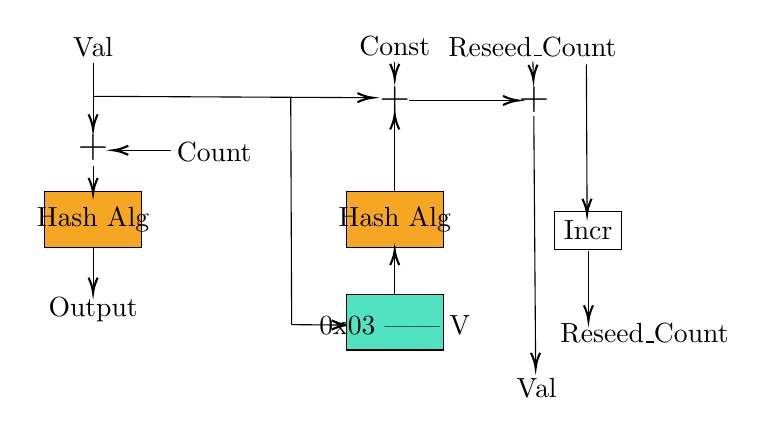
\begin{tikzpicture}[x=1pt,y=1pt,yscale=-0.5,xscale=0.5]
%uncomment if require: \path (0,579); %set diagram left start at 0, and has height of 579

%Shape: Rectangle [id:dp4694514181342362] 
\draw  [fill={rgb, 255:red, 245; green, 166; blue, 35 }  ,fill opacity=1 ] (105.5,126) -- (175.5,126) -- (175.5,166) -- (105.5,166) -- cycle ;
%Straight Lines [id:da4804317787328274] 
\draw    (140.5,33) -- (140.5,79) ;
\draw [shift={(140.5,81)}, rotate = 270] [color={rgb, 255:red, 0; green, 0; blue, 0 }  ][line width=0.75]    (10.93,-3.29) .. controls (6.95,-1.4) and (3.31,-0.3) .. (0,0) .. controls (3.31,0.3) and (6.95,1.4) .. (10.93,3.29)   ;

%Straight Lines [id:da33332051652659533] 
\draw    (140.5,107) -- (140.5,125) ;
\draw [shift={(140.5,127)}, rotate = 270] [color={rgb, 255:red, 0; green, 0; blue, 0 }  ][line width=0.75]    (10.93,-3.29) .. controls (6.95,-1.4) and (3.31,-0.3) .. (0,0) .. controls (3.31,0.3) and (6.95,1.4) .. (10.93,3.29)   ;

%Straight Lines [id:da8888881528784542] 
\draw    (196.5,96) -- (157,96) ;
\draw [shift={(155,96)}, rotate = 360] [color={rgb, 255:red, 0; green, 0; blue, 0 }  ][line width=0.75]    (10.93,-3.29) .. controls (6.95,-1.4) and (3.31,-0.3) .. (0,0) .. controls (3.31,0.3) and (6.95,1.4) .. (10.93,3.29)   ;

%Straight Lines [id:da5662691554074395] 
\draw    (140.5,166) -- (140.5,197) ;
\draw [shift={(140.5,199)}, rotate = 270] [color={rgb, 255:red, 0; green, 0; blue, 0 }  ][line width=0.75]    (10.93,-3.29) .. controls (6.95,-1.4) and (3.31,-0.3) .. (0,0) .. controls (3.31,0.3) and (6.95,1.4) .. (10.93,3.29)   ;

%Straight Lines [id:da6988949604392514] 
\draw    (140.5,57) -- (340.5,57.99) ;
\draw [shift={(342.5,58)}, rotate = 180.28] [color={rgb, 255:red, 0; green, 0; blue, 0 }  ][line width=0.75]    (10.93,-3.29) .. controls (6.95,-1.4) and (3.31,-0.3) .. (0,0) .. controls (3.31,0.3) and (6.95,1.4) .. (10.93,3.29)   ;

%Shape: Rectangle [id:dp14932965513622842] 
\draw  [fill={rgb, 255:red, 245; green, 166; blue, 35 }  ,fill opacity=1 ] (323.5,126) -- (393.5,126) -- (393.5,166) -- (323.5,166) -- cycle ;
%Straight Lines [id:da3396677055374049] 
\draw    (284,222) -- (322,222.32) ;
\draw [shift={(324,222.33)}, rotate = 180.48] [color={rgb, 255:red, 0; green, 0; blue, 0 }  ][line width=0.75]    (10.93,-3.29) .. controls (6.95,-1.4) and (3.31,-0.3) .. (0,0) .. controls (3.31,0.3) and (6.95,1.4) .. (10.93,3.29)   ;

%Straight Lines [id:da42308701192525344] 
\draw    (283.33,58) -- (284,222) ;


%Shape: Rectangle [id:dp89463250951755] 
\draw  [fill={rgb, 255:red, 80; green, 227; blue, 194 }  ,fill opacity=1 ] (323.5,200.33) -- (393.5,200.33) -- (393.5,240.33) -- (323.5,240.33) -- cycle ;
%Straight Lines [id:da49928196364625355] 
\draw    (358.5,200) -- (358.5,170) ;
\draw [shift={(358.5,168)}, rotate = 450] [color={rgb, 255:red, 0; green, 0; blue, 0 }  ][line width=0.75]    (10.93,-3.29) .. controls (6.95,-1.4) and (3.31,-0.3) .. (0,0) .. controls (3.31,0.3) and (6.95,1.4) .. (10.93,3.29)   ;

%Straight Lines [id:da6855931770412393] 
\draw    (358.5,125.33) -- (358.5,72) ;
\draw [shift={(358.5,70)}, rotate = 450] [color={rgb, 255:red, 0; green, 0; blue, 0 }  ][line width=0.75]    (10.93,-3.29) .. controls (6.95,-1.4) and (3.31,-0.3) .. (0,0) .. controls (3.31,0.3) and (6.95,1.4) .. (10.93,3.29)   ;

%Straight Lines [id:da6227737689441111] 
\draw    (369,60) -- (445.67,60) ;
\draw [shift={(447.67,60)}, rotate = 180] [color={rgb, 255:red, 0; green, 0; blue, 0 }  ][line width=0.75]    (10.93,-3.29) .. controls (6.95,-1.4) and (3.31,-0.3) .. (0,0) .. controls (3.31,0.3) and (6.95,1.4) .. (10.93,3.29)   ;

%Straight Lines [id:da6879996099589978] 
\draw    (459,71.33) -- (460.32,251.33) ;
\draw [shift={(460.33,253.33)}, rotate = 269.58] [color={rgb, 255:red, 0; green, 0; blue, 0 }  ][line width=0.75]    (10.93,-3.29) .. controls (6.95,-1.4) and (3.31,-0.3) .. (0,0) .. controls (3.31,0.3) and (6.95,1.4) .. (10.93,3.29)   ;

%Straight Lines [id:da7970345168288206] 
\draw    (497,34) -- (497.49,140) ;
\draw [shift={(497.5,142)}, rotate = 269.73] [color={rgb, 255:red, 0; green, 0; blue, 0 }  ][line width=0.75]    (10.93,-3.29) .. controls (6.95,-1.4) and (3.31,-0.3) .. (0,0) .. controls (3.31,0.3) and (6.95,1.4) .. (10.93,3.29)   ;

%Shape: Rectangle [id:dp10952024955805229] 
\draw   (474,140) -- (522.5,140) -- (522.5,168) -- (474,168) -- cycle ;
%Straight Lines [id:da8266200532258523] 
\draw    (498.5,169) -- (498.5,217) ;
\draw [shift={(498.5,219)}, rotate = 270] [color={rgb, 255:red, 0; green, 0; blue, 0 }  ][line width=0.75]    (10.93,-3.29) .. controls (6.95,-1.4) and (3.31,-0.3) .. (0,0) .. controls (3.31,0.3) and (6.95,1.4) .. (10.93,3.29)   ;


% Text Node
\draw (140.5,21) node  [align=left] {Val};
% Text Node
\draw (358.5,21) node  [align=left] {Const};
% Text Node
\draw (458,21) node  [align=left] {Reseed\_Count};
% Text Node
\draw (140.5,146) node  [align=left] {Hash Alg};
% Text Node
\draw (140.5,94) node  [align=left] {{\Large +}};
% Text Node
\draw (228,97) node  [align=left] {Count};
% Text Node
\draw (140.5,211) node  [align=left] {Output};
% Text Node
\draw (358.5,59) node  [align=left] {{\Large +}};
% Text Node
\draw (358.5,222) node  [align=left] {0x03 || V};
% Text Node
\draw (358.5,146.33) node  [align=left] {Hash Alg};
% Text Node
\draw (459.17,59.67) node  [align=left] {{\Large +}};
% Text Node
\draw (461,268) node  [align=left] {Val};
% Text Node
\draw (498.25,154) node  [align=left] {Incr};
% Text Node
\draw (539,228) node  [align=left] {Reseed\_Count};
% Connection
\draw    (358.5,32) -- (358.5,42.5) ;
\draw [shift={(358.5,44.5)}, rotate = 270] [color={rgb, 255:red, 0; green, 0; blue, 0 }  ][line width=0.75]    (10.93,-3.29) .. controls (6.95,-1.4) and (3.31,-0.3) .. (0,0) .. controls (3.31,0.3) and (6.95,1.4) .. (10.93,3.29)   ;

% Connection
\draw    (458.33,32) -- (458.67,43.17) ;
\draw [shift={(458.73,45.17)}, rotate = 268.27] [color={rgb, 255:red, 0; green, 0; blue, 0 }  ][line width=0.75]    (10.93,-3.29) .. controls (6.95,-1.4) and (3.31,-0.3) .. (0,0) .. controls (3.31,0.3) and (6.95,1.4) .. (10.93,3.29)   ;

\end{tikzpicture}
\caption{Hash Based DRBG Flow for Bit Generation Request~\cite{barker2015nist90a}}
\label{fig:DRBG}
\end{figure}

When a hash-based DRGB is instantiated several steps of setup are required~\cite{barker2015nist90a}. First the true seed is calculated as a hash of \\$entropyInput || nonce || personalizationString$ with the persionalization string being optional. This seed is set to the initial value of the DRGB internal state. The constant is then generated by hashing the seed with a byte of zeros preceding it. Finally, the reseed count is set to 1. 

When random data is requested the current value gets added to an internal counter which is initially zero (see Figure \ref{fig:DRBG}). This is then hashed to generate an output block of bits. If more bits were requested then the internal counter is incremented and the next set of bits is generated. This proceeds until the correct number of bits have been returned. Then to update the value for the next run it is concatenated to 0x03 and hashed. This is added to the initial value and the constant. Finally this is added to the reseed counter to get the value to use for the next random bit generation. 

By generating output bits in this way it is known that this is a deterministic process and because of the one-way function of hash algorithms the bits generated would be sufficiently hard to guess without knowledge of the system's state~\cite{chang2006indifferentiable}. 

\begin{table}[ht]
\begin{tabular}{c|ccc}
                                                                        & \textbf{SHA-1} & \textbf{SHA-256} & \textbf{SHA-512} \\ \hline
\textbf{Security Strength}                                              & 128            & 256              & 256              \\
\textbf{\begin{tabular}[c]{@{}c@{}}Output Block\\ Length\end{tabular}}  & 160            & 256              & 512              \\
\textbf{Seed Length}                                                    & 440            & 440              & 888              \\
\textbf{\begin{tabular}[c]{@{}c@{}}Max Bits per\\ Request\end{tabular}} & $\leq 2^{19}$    & $\leq 2^{19}$      & $\leq 2^{19}$      \\
\textbf{Reseed Interval}                                                & $\leq 2^{48}$    & $\leq 2^{48}$      & $\leq 2^{48}$     
\end{tabular}
\caption{Summary of Hash Based DRBG Properties}
\label{tbl:DRGB_Hash}
\end{table}

\subsection{Uncoordinated Frequency Hopping}

We have previously covered methods mitigating jamming attacks. However, in this section we will perform a more in depth look at jamming resistant key exchange (JRKE) through uncoordinated frequency hopping (UFH)~\cite{strasser2008jamming}. We do this because our proposed solution uses it as the method of establishing a shared secret which is pivotal for the successful mitigation of jamming attacks. 

Most schemes of jamming resistance rely on the two parties holding a shared secret which they can use in a way which coordinates their efforts to circumvent the jammer's malicious efforts. However, in purely wireless systems this proves to be a circular dependency; it is difficult to establish a shared secret over a jammed channel, so the parties switch to using a jamming resistant protocol, but the parties then need to establish a shared secret for this to work. JRKE through UFH seeks to eliminate this redundancy by eliminating the need for the parties to hold a shared secret between them. 

Uncoordinated frequency hopping is a method of avoiding jamming by randomly switching the channels which is being transmitted and listened on. As shown in figure \ref{fig:UFH_rand_channels} each time a message is transmitted there is a small but positive chance that the receiver is listening on the same channel. If this is the case then that packet of the message has been successfully received. However, because of the low probability of a packet being receiver at any given time it is necessary to resend the message many times to ensure with a high likely-hood that the receiver saw each packet of the message. By transmitting in this way it prevents the jammer from being able to jam a single channel and forces them to either engage in costly multi-channel jamming or switch attack methods. 

\begin{figure}[ht]
    \centering

    \tikzset{every picture/.style={line width=0.75pt}} %set default line width to 0.75pt        
    
    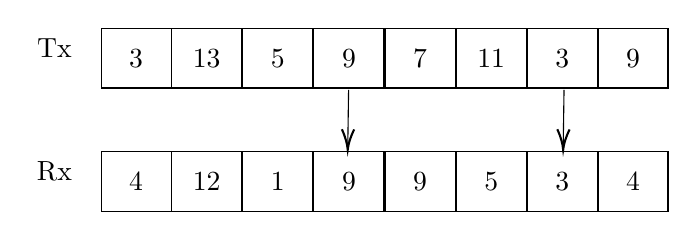
\begin{tikzpicture}[x=0.75pt,y=0.75pt,yscale=-0.9,xscale=0.9]
    %uncomment if require: \path (0,579); %set diagram left start at 0, and has height of 579
    
    %Shape: Rectangle [id:dp21390468484872693] 
    \draw   (79.5,35) -- (117,35) -- (117,67) -- (79.5,67) -- cycle ;
    
    %Shape: Rectangle [id:dp194781887570034] 
    \draw   (117.29,35) -- (154.79,35) -- (154.79,67) -- (117.29,67) -- cycle ;
    
    %Shape: Rectangle [id:dp8903064451015634] 
    \draw   (193.45,35) -- (230.95,35) -- (230.95,67) -- (193.45,67) -- cycle ;
    
    %Shape: Rectangle [id:dp2111774092369394] 
    \draw   (155.37,35) -- (192.87,35) -- (192.87,67) -- (155.37,67) -- cycle ;
    
    %Shape: Rectangle [id:dp790158940095278] 
    \draw   (231.53,35) -- (269.03,35) -- (269.03,67) -- (231.53,67) -- cycle ;
    
    %Shape: Rectangle [id:dp19056199375219807] 
    \draw   (269.61,35) -- (307.11,35) -- (307.11,67) -- (269.61,67) -- cycle ;
    
    %Shape: Rectangle [id:dp6973758187774042] 
    \draw   (345.5,35) -- (383,35) -- (383,67) -- (345.5,67) -- cycle ;
    
    %Shape: Rectangle [id:dp16120774737598786] 
    \draw   (307.69,35) -- (345.19,35) -- (345.19,67) -- (307.69,67) -- cycle ;
    
    
    %Shape: Rectangle [id:dp010481494864986951] 
    \draw   (79.5,101) -- (117,101) -- (117,133) -- (79.5,133) -- cycle ;
    
    %Shape: Rectangle [id:dp3223336933867067] 
    \draw   (117.29,101) -- (154.79,101) -- (154.79,133) -- (117.29,133) -- cycle ;
    
    %Shape: Rectangle [id:dp0950704395037203] 
    \draw   (193.45,101) -- (230.95,101) -- (230.95,133) -- (193.45,133) -- cycle ;
    
    %Shape: Rectangle [id:dp6298336606158916] 
    \draw   (155.37,101) -- (192.87,101) -- (192.87,133) -- (155.37,133) -- cycle ;
    
    %Shape: Rectangle [id:dp07910296159143915] 
    \draw   (231.53,101) -- (269.03,101) -- (269.03,133) -- (231.53,133) -- cycle ;
    
    %Shape: Rectangle [id:dp7742135888615012] 
    \draw   (269.61,101) -- (307.11,101) -- (307.11,133) -- (269.61,133) -- cycle ;
    
    %Shape: Rectangle [id:dp06720198488620577] 
    \draw   (345.5,101) -- (383,101) -- (383,133) -- (345.5,133) -- cycle ;
    
    %Shape: Rectangle [id:dp7638983485937891] 
    \draw   (307.69,101) -- (345.19,101) -- (345.19,133) -- (307.69,133) -- cycle ;
    
    
    %Straight Lines [id:da01879080885393325] 
    \draw    (212,68) -- (211.56,98.07) ;
    \draw [shift={(211.53,100.07)}, rotate = 270.85] [color={rgb, 255:red, 0; green, 0; blue, 0 }  ][line width=0.75]    (10.93,-3.29) .. controls (6.95,-1.4) and (3.31,-0.3) .. (0,0) .. controls (3.31,0.3) and (6.95,1.4) .. (10.93,3.29)   ;
    
    %Straight Lines [id:da8852534803330441] 
    \draw    (327.33,68) -- (326.89,98.07) ;
    \draw [shift={(326.86,100.07)}, rotate = 270.85] [color={rgb, 255:red, 0; green, 0; blue, 0 }  ][line width=0.75]    (10.93,-3.29) .. controls (6.95,-1.4) and (3.31,-0.3) .. (0,0) .. controls (3.31,0.3) and (6.95,1.4) .. (10.93,3.29)   ;
    
    
    % Text Node
    \draw (98.25,51) node  [align=left] {3};
    % Text Node
    \draw (212.2,51) node  [align=left] {9};
    % Text Node
    \draw (136.04,51) node  [align=left] {13};
    % Text Node
    \draw (174.12,51) node  [align=left] {5};
    % Text Node
    \draw (326.44,51) node  [align=left] {3};
    % Text Node
    \draw (364.25,51) node  [align=left] {9};
    % Text Node
    \draw (288.36,51) node  [align=left] {11};
    % Text Node
    \draw (250.28,51) node  [align=left] {7};
    % Text Node
    \draw (54.5,45.5) node  [align=left] {Tx};
    % Text Node
    \draw (54.5,111.5) node  [align=left] {Rx};
    % Text Node
    \draw (326.44,117) node  [align=left] {3};
    % Text Node
    \draw (364.25,117) node  [align=left] {4};
    % Text Node
    \draw (288.36,117) node  [align=left] {5};
    % Text Node
    \draw (250.28,117) node  [align=left] {9};
    % Text Node
    \draw (174.12,117) node  [align=left] {1};
    % Text Node
    \draw (212.2,117) node  [align=left] {9};
    % Text Node
    \draw (136.04,117) node  [align=left] {12};
    % Text Node
    \draw (98.25,117) node  [align=left] {4};
    
    
    \end{tikzpicture}
    
    \caption{Uncoordinated Frequency Hopping Packet Transfer}
    \label{fig:UFH_rand_channels}
\end{figure}

On its own this method of UFH works to allow the transmission of data around a jammer. However, it does not prevent the attacker from inserting their data within valid transmissions from the sender. To this end a hash-link chain has been developed to allow JRKE over UFH to avoid an attacker from inserting malicious data into an otherwise valid packet. Each packet sent contains an $id$ which is used to identify the message sequence, a packet number used to identify the order of the packets since it is not guaranteed that the packets will arrive in order, a portion of the message data, and a hash of the next packet's message data (see Figure \ref{fig:UFH_hash}). By linking the message fragments in this way it is possible to ensure the packets which are present in this chain are the packets that are intended to be there.

\begin{figure}[ht]
    \centering

    \tikzset{every picture/.style={line width=0.75pt}} %set default line width to 0.75pt        
    
    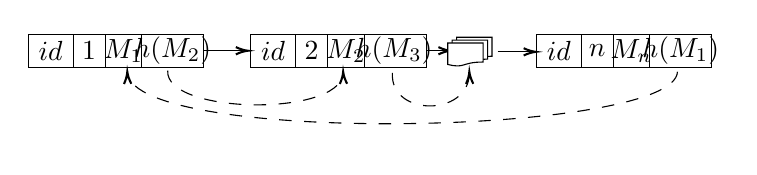
\begin{tikzpicture}[x=1pt,y=1pt,yscale=-0.4,xscale=0.4]
    %uncomment if require: \path (0,579); %set diagram left start at 0, and has height of 579
    
    %Shape: Rectangle [id:dp23224882883476283] 
    \draw   (30,14) -- (70.5,14) -- (70.5,44) -- (30,44) -- cycle ;
    %Shape: Rectangle [id:dp6687621231702099] 
    \draw   (70.5,14) -- (99.5,14) -- (99.5,44) -- (70.5,44) -- cycle ;
    %Shape: Rectangle [id:dp15262267073484748] 
    \draw   (99.5,14) -- (132.5,14) -- (132.5,44) -- (99.5,44) -- cycle ;
    %Shape: Rectangle [id:dp18689516582204613] 
    \draw   (132.5,14) -- (188.5,14) -- (188.5,44) -- (132.5,44) -- cycle ;
    
    %Shape: Rectangle [id:dp2617611850582511] 
    \draw   (231,14) -- (271.5,14) -- (271.5,44) -- (231,44) -- cycle ;
    %Shape: Rectangle [id:dp07899681119772306] 
    \draw   (271.5,14) -- (300.5,14) -- (300.5,44) -- (271.5,44) -- cycle ;
    %Shape: Rectangle [id:dp8460068179559377] 
    \draw   (300.5,14) -- (333.5,14) -- (333.5,44) -- (300.5,44) -- cycle ;
    %Shape: Rectangle [id:dp883716724147019] 
    \draw   (333.5,14) -- (389.5,14) -- (389.5,44) -- (333.5,44) -- cycle ;
    
    %Shape: Rectangle [id:dp6205658045352709] 
    \draw   (489,14) -- (529.5,14) -- (529.5,44) -- (489,44) -- cycle ;
    %Shape: Rectangle [id:dp9897702069238967] 
    \draw   (529.5,14) -- (558.5,14) -- (558.5,44) -- (529.5,44) -- cycle ;
    %Shape: Rectangle [id:dp753999428232139] 
    \draw   (558.5,14) -- (591.5,14) -- (591.5,44) -- (558.5,44) -- cycle ;
    %Shape: Rectangle [id:dp04669871534113401] 
    \draw   (591.5,14) -- (647.5,14) -- (647.5,44) -- (591.5,44) -- cycle ;
    
    %Straight Lines [id:da5089415901312635] 
    \draw    (189,29) -- (226.5,29) ;
    \draw [shift={(228.5,29)}, rotate = 180] [color={rgb, 255:red, 0; green, 0; blue, 0 }  ][line width=0.75]    (10.93,-3.29) .. controls (6.95,-1.4) and (3.31,-0.3) .. (0,0) .. controls (3.31,0.3) and (6.95,1.4) .. (10.93,3.29)   ;
    
    %Straight Lines [id:da36251774501746215] 
    \draw    (390,29) -- (409.5,29) ;
    \draw [shift={(411.5,29)}, rotate = 180] [color={rgb, 255:red, 0; green, 0; blue, 0 }  ][line width=0.75]    (10.93,-3.29) .. controls (6.95,-1.4) and (3.31,-0.3) .. (0,0) .. controls (3.31,0.3) and (6.95,1.4) .. (10.93,3.29)   ;
    
    %Straight Lines [id:da3847890586773832] 
    \draw    (454,30) -- (486.5,30) ;
    \draw [shift={(488.5,30)}, rotate = 180] [color={rgb, 255:red, 0; green, 0; blue, 0 }  ][line width=0.75]    (10.93,-3.29) .. controls (6.95,-1.4) and (3.31,-0.3) .. (0,0) .. controls (3.31,0.3) and (6.95,1.4) .. (10.93,3.29)   ;
    
    %Flowchart: Multidocument [id:dp05645253073998391] 
    \draw  [fill={rgb, 255:red, 255; green, 255; blue, 255 }  ,fill opacity=1 ] (417,16.84) -- (449,16.84) -- (449,34) .. controls (429,34) and (433,40.19) .. (417,36.18) -- cycle ; \draw  [fill={rgb, 255:red, 255; green, 255; blue, 255 }  ,fill opacity=1 ] (413,19.44) -- (445,19.44) -- (445,36.6) .. controls (425,36.6) and (429,42.79) .. (413,38.78) -- cycle ; \draw  [fill={rgb, 255:red, 255; green, 255; blue, 255 }  ,fill opacity=1 ] (409,22.04) -- (441,22.04) -- (441,39.2) .. controls (421,39.2) and (425,45.39) .. (409,41.38) -- cycle ;
    %Curve Lines [id:da38806950432906295] 
    \draw  [dash pattern={on 4.5pt off 4.5pt}]  (156,47) .. controls (153.54,86.4) and (310.68,88.93) .. (314.44,49.82) ;
    \draw [shift={(314.5,48)}, rotate = 448.6] [color={rgb, 255:red, 0; green, 0; blue, 0 }  ][line width=0.75]    (10.93,-3.29) .. controls (6.95,-1.4) and (3.31,-0.3) .. (0,0) .. controls (3.31,0.3) and (6.95,1.4) .. (10.93,3.29)   ;
    
    %Curve Lines [id:da8227290809698264] 
    \draw  [dash pattern={on 4.5pt off 4.5pt}]  (359,49) .. controls (356.54,88.4) and (427.33,88.99) .. (428.5,49.82) ;
    \draw [shift={(428.5,48)}, rotate = 448.6] [color={rgb, 255:red, 0; green, 0; blue, 0 }  ][line width=0.75]    (10.93,-3.29) .. controls (6.95,-1.4) and (3.31,-0.3) .. (0,0) .. controls (3.31,0.3) and (6.95,1.4) .. (10.93,3.29)   ;
    
    %Curve Lines [id:da5951392950706831] 
    \draw  [dash pattern={on 4.5pt off 4.5pt}]  (616.5,48) .. controls (614.51,105.71) and (126.42,114.91) .. (119.57,49) ;
    \draw [shift={(119.5,48)}, rotate = 448.29] [color={rgb, 255:red, 0; green, 0; blue, 0 }  ][line width=0.75]    (10.93,-3.29) .. controls (6.95,-1.4) and (3.31,-0.3) .. (0,0) .. controls (3.31,0.3) and (6.95,1.4) .. (10.93,3.29)   ;
    
    
    % Text Node
    \draw (160.5,29) node   {$h( M_{2})$};
    % Text Node
    \draw (50.25,29) node   {$id$};
    % Text Node
    \draw (85,29) node   {$1$};
    % Text Node
    \draw (116,29) node   {$M_{1}$};
    % Text Node
    \draw (360.5,29) node   {$h( M_{3})$};
    % Text Node
    \draw (251.25,29) node   {$id$};
    % Text Node
    \draw (286,29) node   {$2$};
    % Text Node
    \draw (317,29) node   {$M_{2}$};
    % Text Node
    \draw (619.5,29) node   {$h( M_{1})$};
    % Text Node
    \draw (509.25,29) node   {$id$};
    % Text Node
    \draw (544,29) node   {$n$};
    % Text Node
    \draw (575,29) node   {$M_{n}$};
    
    
    \end{tikzpicture}
    
    \caption{JRKE through UFH Hash-Link Chain~\cite{strasser2008jamming}}
    \label{fig:UFH_hash}
\end{figure}

However, a smart attacker may attempt to send entire malicious packets. JRKE through UFH does not inherently provided a method of preventing this behaviour. However, the key exchange used is not fixed and there are key-exchange methods which provide packet validation through a variety of methods such as certificates and packet signing. This is just one method and the actual prevention of packet spoofing is left to the implementer to choose what is considered a sufficiently secure key-exchange algorithm.

\section{Jelly Interleaver Design}
\label{sec:interleaver_design}

In this section, we describe our suggested approach to mitigating interleaver targeted jamming. As suggested by Vo-Huu et al. we use a shared secret between the transmitter and receiver in order to cryptographically randomize the underlying interleaving pattern~\cite{vo2016interleaving}. This prohibits the attack of specific sub-carriers in order to create post de-interleaving jamming. This shared secret is determined and shared at connection time through uncoordinated frequency hopping. 

The rest of this section will be organized as follows. We will first discuss the additional steps required to establish a connection in section \ref{sub:setup}. In section \ref{sub:interleavingAlg} we will then discuss the modified interleaving algorithm, with section \ref{sub:deinterleave} discussing the de-interleaving mechanism. Finally, we perform an analytic analysis of Jelly interleaving in section \ref{sub:analyticAnalysis}.

\subsection{Modified Connection Setup}
\label{sub:setup}

IEEE 802.11 specifies a specific handshake used to establish a secure connection between the transmitter and receiver. In order to do this it sends packets over the air using the default interleaver~\cite{cooklev2004wireless}. This means these packets are also subjected to interleaver targeted jamming. Because of this a jammer could feasibly prevent any connection from ever being established. In order to establish the modified interleaver we propose in section \ref{sub:interleavingAlg} a secret needs to be shared between the two parties. Using traditionally interleaved packets for this task is again insufficient as these packets are likely to be jammed by a sufficiently motivated attacker. 

In order to send and generate a shared secret seed between the two we proposed the use of UFH, as shown in figure \ref{fig:connectionProcess}. When a connection attempt is detected UFH and a secure key-exchange protocol should be used in order generate a shared secret key (note that it is not necessary for forward secrecy as we are only prevent real-time attacks). Then continuing to use UFH for our packet delivery we use the secret key to securely share sufficiently random data in order act as a seed for our DRBG. Because there are cases where the receiver and transmitter may not trust each other we propose two methods of exchanging high-entropy data. The first can be used where both parties claim to be concerned with the reliability of the channel. In this case both parties generate a bit string long enough to sufficiently seed the DRBG and the two of these strings are concatenated an used to seed the DRBG. The second method is when only one party claims to care about the reliability of the channel. In this case that party generates the bit stream and it is used without additional modification. 

After the shared secret random seed has been established between the two ends, the interleaving algorithm described below is use to generate a well conditioned and random interleaving pattern. Now that the interleaver is no long vulnerable to targeted jamming, the traditional WiFi handshake can occur without concern of this method of jamming. This process will increase the time required for setup however it is necessary to prevent targeted jamming because of the slower transfer rate of UFH~\cite{strasser2008jamming}.

% Define block styles for flow chart
\tikzstyle{decision} = [diamond, draw, fill=blue!20, 
    text width=4.5em, text badly centered, node distance=3cm, inner sep=0pt]
\tikzstyle{block} = [rectangle, draw, fill=blue!20, 
    text width=5em, text centered, rounded corners, minimum height=4em]
\tikzstyle{connection} = [rectangle, draw, fill=green!20, 
    text width=5em, text centered, rounded corners, minimum height=4em]
\tikzstyle{line} = [draw, -latex']
\tikzstyle{connectionRequest} = [draw, ellipse,fill=red!20, node distance=3cm,
    minimum height=2em]

\begin{figure}[ht]
    \begin{tikzpicture}[node distance = 2cm, auto]
        \node [connectionRequest] (init) {Connection Attempt};
        \node [block, below of=init] (ufh) {Use UFH to Shared Secret Key};
        \node [block, below of=ufh] (secret) {Use UFH to Share Random Seed};
        \node [block, below of=secret, node distance=2.25cm] (initDRBG) {Initialize Deterministic Random Bit Generator};
        \node [block, below of=initDRBG] (dscOffsets) {Generate DSC Offsets};
        \node [decision, below of=dscOffsets] (conditioned) {Are DSC Offsets Well Conditioned?};
        \node [block, right of=conditioned, node distance=2.75cm] (recondition) {Clear DSC Offsets};
        \node [connection, below of=conditioned, node distance=2.75cm] (connected) {Interleaver Ready};
        % Lines
        \path [line] (init) -- (ufh);
        \path [line] (ufh) -- (secret);
        \path [line] (secret) -- (initDRBG);
        \path [line] (initDRBG) -- (dscOffsets);
        \path [line] (dscOffsets) -- (conditioned);
        \path [line] (conditioned) -- node [near start] {No} (recondition);
        \path [line] (recondition) |- (dscOffsets);
        \path [line] (conditioned) -- node {Yes} (connected);
    \end{tikzpicture}
    \caption{Interleaver Connection Process}
    \label{fig:connectionProcess}
\end{figure}

\subsection{Interleaving Algorithm}
\label{sub:interleavingAlg}

In this section we discuss our proposed modification to the IEEE 802.11 interleaving scheme in order to mitigate interleaver targeted jamming attacks. From our UFH intial connection we we able to establish a DRBG which uses the same random seed on both sides of the communication channel. We divide our interleaver modifications into two separate stages: sub-carrier pattern generation and interleaving.

In the DSC pattern generation stage, as shown in Algorithm \ref{alg:patterngen}, we seek to use the DRBG to establish DSC offsets used to perform the interleaving later. To this end we generate a random DSC offset from between 1 and the number of data sub-carriers, inclusive. We then check that this value was not already present in the DSC offset pattern. If it is not present then we append this value to the DSC offset pattern. If it was already present then we simply regenerate a new DSC offset. Once we have a unique offset value for each bit within the sub-carrier, we perform a Fisher-Yates shuffle over the pattern to generate the final pattern~\cite{fisher1943statistical}. It is then necessary to check that pattern is well conditioned to be an interleaver. This is done by ensuring there are no two values in the pattern which are adjacent sub-carriers, so there is at-least a sub-carrier worth of buffer between bits within the same initial DSC. If the pattern is not well conditioned we attempt to generate another patter using the DRBG in its current state. This continues until we find a sufficiently conditioned pattern or the DRBG exceeds its reseed interval at which point we share a new random seed between the two parties and continue.

\begin{algorithm}[ht]
\caption{DSC Interleaver Pattern Generator Algorithm}
\label{alg:patterngen}
\begin{algorithmic}

\REQUIRE $bpsc \in \{1,2,4,6,8\}$
\STATE $DSCoffsets \leftarrow $ Empty Array of Size $bpsc$
\STATE $i \leftarrow 1$
\STATE

\WHILE{$i \leq bpsc$}
    \STATE $randBits \leftarrow DRBG$
    \STATE $randDSC \leftarrow \lceil numSubCarriers * randBits / maxRandVal \rceil$
    \IF{$randDSC \notin DSCoffsets$}
        \STATE $DSCoffsets[i] \leftarrow randDSC$
        \STATE $i \leftarrow i + 1$
    \ENDIF
\ENDWHILE
\STATE

\STATE fisherYatesShuffle($DSCoffsets$)
\STATE 

\ENSURE $\forall i,j \in [1, bpsc], i < j:$ \\ $|DSCoffsets[i]-DSCoffsets[j]| \neq 1$
%\ENSURE $\forall i \in [1,bpsc), |DSCoffsets[i]-DSCoffsets[i+1]| \neq 1 $
%\ENSURE $\forall i \in [1,bpsc-1), |DSCoffsets[i]-DSCoffsets[i+2]| \neq 1 $
%\ENSURE $|DSCoffsets[1]-DSCoffsets[bpsc]| \neq 1$
%\ENSURE $|DSCoffsets[1]-DSCoffsets[bpsc - 1]| \neq 1$
%\ENSURE $|DSCoffsets[2]-DSCoffsets[bpsc]| \neq 1$
\RETURN DSCoffsets
\end{algorithmic}
\end{algorithm}

Generating a DSC pattern only needs to be done once per connection. For improved security this pattern should time-out and be re-computed occasionally. After it has been established it can be used to perform the actual interleaving. We first divide the input stream into a 2D array of bits where each row represents a DSC and each column represents all the values at the particular index of each initial sub-carrier. Then the transformation performs a circular shift on each row where the shift distance is determined by the value in the corresponding position of the DSC pattern. This can be more linearly thought of as shifing each bit within each sub-carrier by the DSC pattern offset in the corresponding position, as we show in Algorithm \ref{alg:interleaving}. Because of the minimal computation requirements after initially generating the DSC pattern this algorithm has the potential to be implemented in hardware and operate at high speeds.

\begin{algorithm}[ht]
\caption{Bit Interleaver Algorithm}
\label{alg:interleaving}
\begin{algorithmic}

\REQUIRE $inputBits \equiv$ 2D Array of Size $bpsc$ X $dataSubCarriers$
\STATE $outputBits \leftarrow $ Empty 2D Array of Size $bpsc$ X $dataSubCarriers$
\STATE

\FOR{$b \in [1, bpsc]$}
    \FOR{$d \in [1, dataSubCarriers]$}
        \STATE $newDSC \leftarrow mod((d + DSCoffsets[b]), dataSubCarriers)$
        \STATE $outputBits[b][newDSC] \leftarrow inputBits[b][d]$
    \ENDFOR
\ENDFOR
\STATE

\RETURN outputBits 
\end{algorithmic}
\end{algorithm}



\subsection{De-Interleaving}
\label{sub:deinterleave}

Our interleaving algorithm shifts the bit in each position by a certain value, so we are able to re-establish the original bit stream by pulling each bit from its final location. We show this in Algorithm \ref{alg:deinterleaving}.

\begin{algorithm}[ht]
\caption{Bit De-Interleaver Algorithm}
\label{alg:deinterleaving}
\begin{algorithmic}

\REQUIRE $inputBits \equiv$ 2D Array of Size $bpsc$ X $dataSubCarriers$
\STATE $outputBits \leftarrow $ Empty 2D Array of Size $bpsc$ X $dataSubCarriers$
\STATE

\FOR{$b \in [1, bpsc]$}
    \FOR{$d \in [1, dataSubCarriers]$}
        \STATE $oldDSC \leftarrow mod((d + DSCoffsets[b]), dataSubCarriers)$
        \STATE $outputBits[b][d] \leftarrow inputBits[b][oldDSC]$
    \ENDFOR
\ENDFOR
\STATE

\RETURN outputBits 
\end{algorithmic}
\end{algorithm}


\subsection{Analytic Analysis of Interleaving Patterns}
\label{sub:analyticAnalysis}

There are several tasks which an interleaver must achieve in order to be successful before we are able to evaluate the security of the system against targeted attacks. To this end, we ensure that our interleaver will provide protection against bursty errors on a given frequency. This is done by checking that the data sub-carrier offsets generated through the interleaving pattern generator algorithm are at least two sub-carriers apart for bits which are initially within the same sub-carrier. This means we can guarantee that there is a sub-carrier buffer between these so the noisy burst would have to span over an entire sub-carriers which is 312.5 KHz in 802.11's scheme of OFDM~\cite{ieee80211}. Additionally, interleavers for OFDM need to shuffle adjacent bits so they do not share the same position in sub-carriers. This is necessary to combat any bias distortion which could occur over the same bit of different sub-carrier OFDM. Our proposed interleaver naturally does this by leaving the bits in the same position within their shifted data sub-carrier as they were in their initial sub-carrier. Through this qualitative analysis it is possible to show that our interleaving mechanism meets these minimal requirements as an effective interleaver.

Of equal concern is the security of this design against malicious attacks. We explore the security levels of each component within our design in the remainder of this section.

The first potential attack surface in our design is the process of using UFH to generate a shared secret which is then used to seed the DRBG. There are two main attacks we consider on this front: man-in-the-middle and secret leakage. Both of these would allow the attacker to determine a subset of sub-carriers which could be targeted to perform the same jamming effect. Strasser et al. were able to show that because of the nature of the hash-link chains used in UFH it becomes exponentially difficult for an attacker to insert or modify data within an individual message chain because of the difficulty in finding a hash collision for the a proceeding packet~\cite{strasser2008jamming}. This is only as secure as the hash algorithm, but it is known that SHA-256 has a security level of 128 bits so this is not a vulnerability in the system against current computation resources~\cite{barker2016nist57}. However, UFH does not prevent against the malicious delivery or reception of packets during the key exchange performed over it. This must be accounted for within the key-exchange protocol. This is a solved problem and can be overcome by using digital signatures for authentication, time-stamps for freshness, and a strong key exchange such as Elliptic Curve Cryptography with the Diffie-Hellman key exchange for example~\cite{canetti2001analysis, xie2017provably}.

The next attack surface is the randomness of the shared secret and the security of the DRBG. The entropy of the shared secret is a difficult problem as it requires the generator to be truthful about their entropy. It is for this reason we proposed two methods of generating the shared secret. This allows the parties which claim to be concerned with the jamming resistance for the connection to contribute to the shared secret so they only need to trust themselves. In terms of the security of the DRBG, NIST further discusses the security considerations of each type of DRBG in SP800-90a revision 1~\cite{barker2015nist90a}. Our implementation used the Hash-based DRNBG with SHA underlying and NIST considers this as secure as the digest size of the particular hash (up to 256 bits of security). 

The final potential attack surface is the set of possible interleaver configurations. If this number were small it would be substantially more likely for an attacker to be able to randomly guess the interleaver configuration. To ensure the security we now show the number of possible configurations is large enough to not pose a security concern. We again let $b$ be the number of bits per sub-carrier and we use 48 data sub-carriers as is standard for 802.11. We start by determining the number of unconditioned possibilities. This number is fairly small for BPSK and QPSK ($b= 1$ and $2$ respectively), however it grows much larger for QAM. We now must determine the number of combinations which do not meet our conditioning requirements.
%(see Appendix \ref{ap:proof_lower_bound} for proof). 
$$N \geq \prod_{i=0}^{b-1} 48 - 3*i$$
Note that this is a strict lower bound on the number of possible combinations. Using this bound we find the number of unique configurations to be larger than 3,538,080 and 4,203,239,040 for 16QAM and 64QAM respectively.  This provides an adequately large search space so that an attack is unlikely to properly choose the correct configuration at random.

\section{Testing Method}
\label{sec:testing}

For testing our modified interleaving mechanism we sought to stay close to the testing procedure of the initial attack paper by Vo-Huu et al. in order to obtain consistent results~\cite{vo2016interleaving}. To this end we obtained the source code used by the attack paper to generate the jamming signal on a HackRF~\cite{vo2016software}. In this section, we discuss our testing procedure.

For our transmitter and receiver we used software defined radio as the interleaver is most often a hardware component and we needed to modify it. We elected to use the \textit{gr-ieee802-11} implementation for GNU-Radio because of its open source nature and relatively high speeds~\cite{gr_ieee802}. We modified the underlying implementation to use our design with a fixed specified shared secret. We did not elect to perform the secret sharing and initialization because it is beyond the scope of this paper and there are other publications which have already explored that topic. 

Our implementation for testing used a SHA-256 hash-based DRBG as our deterministic source of randomness. Over the course of testing we tested across 30 different initial seeds which were randomly generated using \textit{/dev/random} as our source of entropy. 

A HackRF with the provided attack firmware was used as our jamming device, with SDRs for both our transmitter and reciever. All three of these devices were linked through SMA and a T-junction as shown in Figure \ref{fig:test_setup} and \ref{fig:test_setup_diagram}.

\begin{figure}[ht]
    \centering
    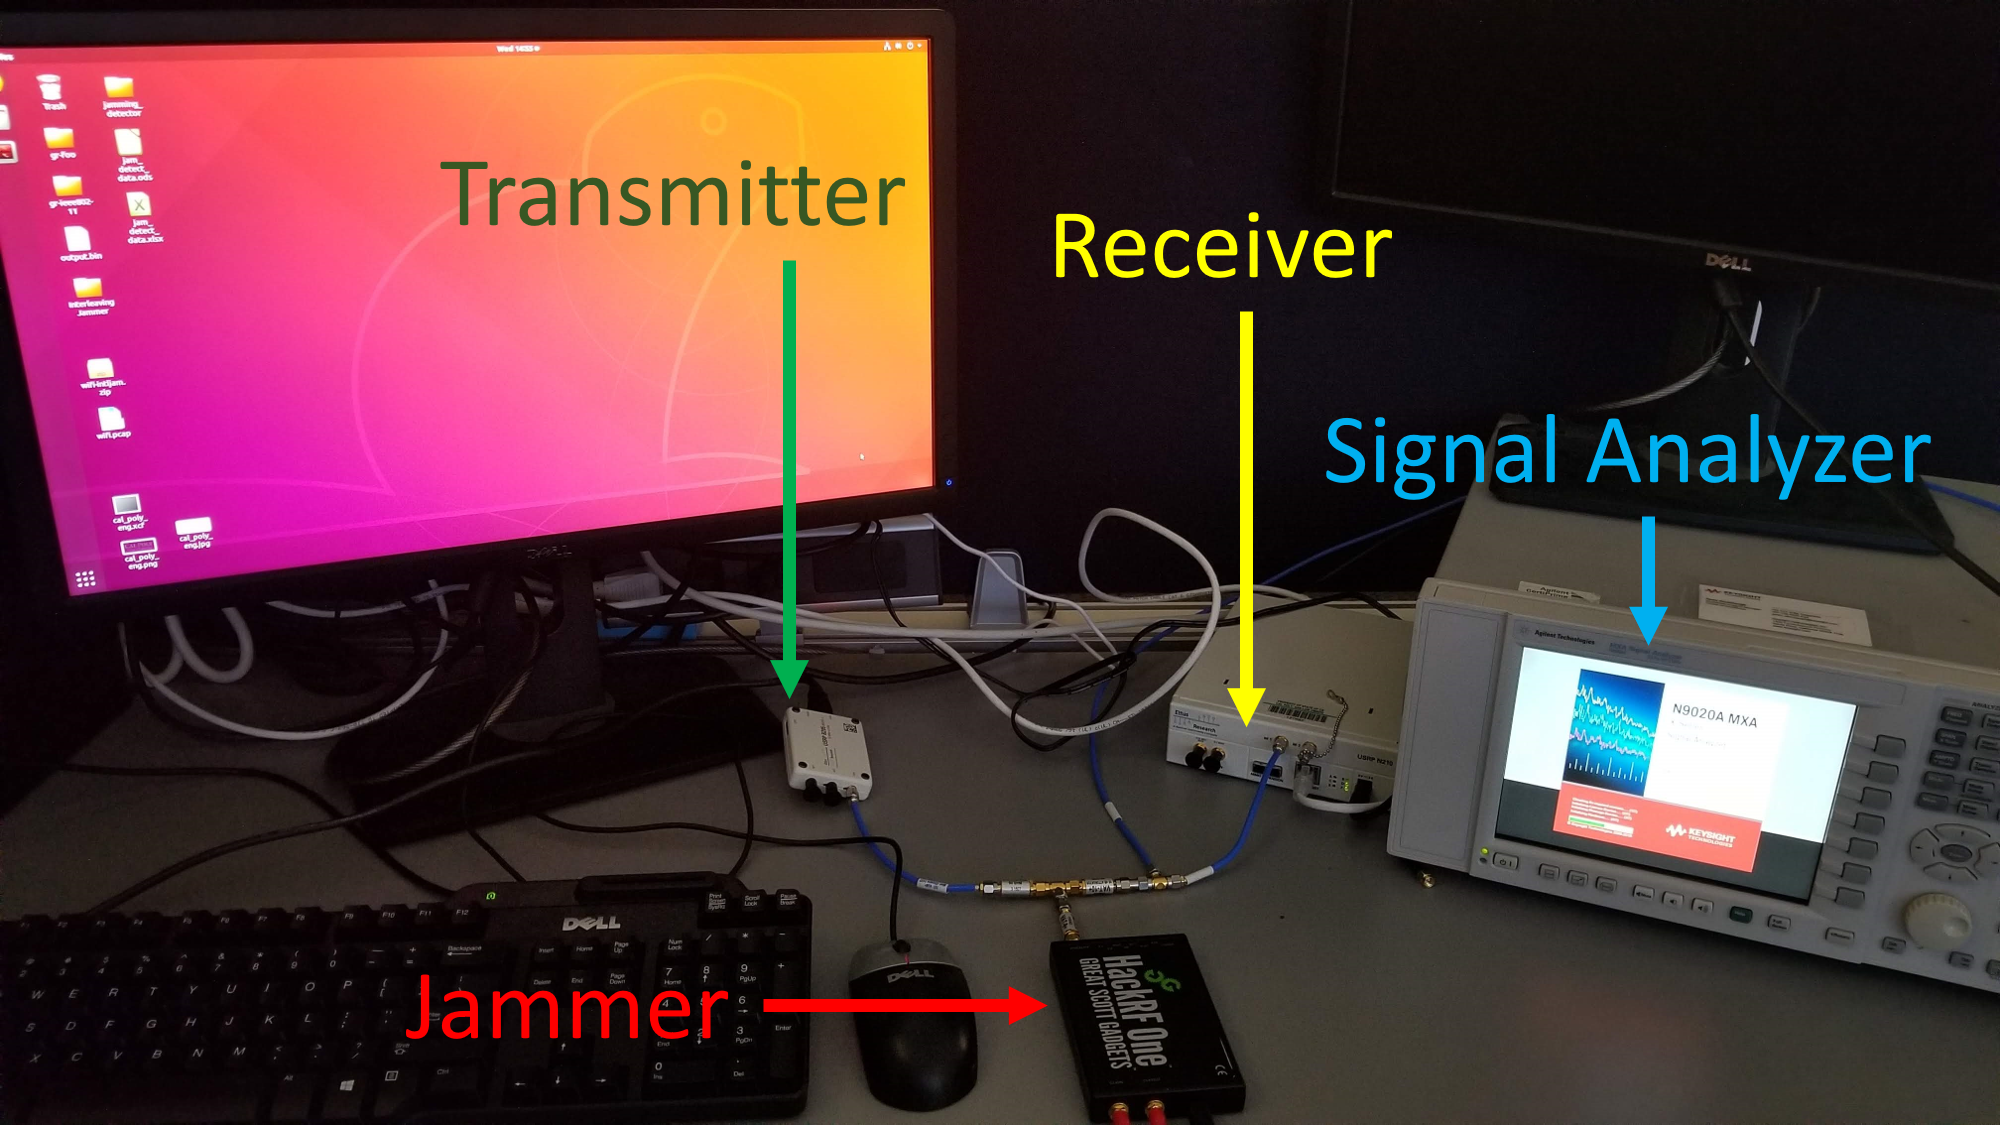
\includegraphics[width=\linewidth]{testing_setup.png}
    \caption{In this figure, we show our test bench setup used for testing the Jelly Interleaver.  }
    \label{fig:test_setup}
\end{figure}

\begin{figure}[ht]
    \centering

    \tikzset{every picture/.style={line width=0.75pt}} %set default line width to 0.75pt        
    
    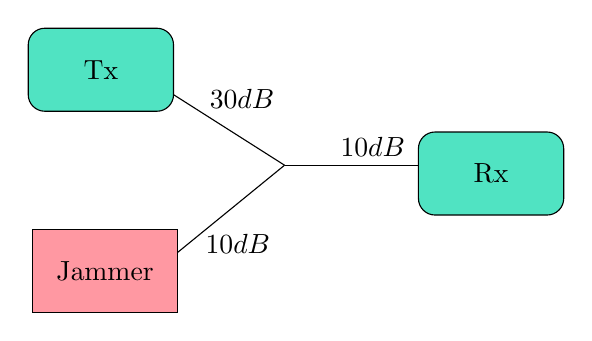
\begin{tikzpicture}[x=0.75pt,y=0.75pt,yscale=-1,xscale=1]
    %uncomment if require: \path (0,579); %set diagram left start at 0, and has height of 579
    
    %Rounded Rect [id:dp03595250693405627] 
    \draw  [fill={rgb, 255:red, 80; green, 227; blue, 194 }  ,fill opacity=1 ] (20,19) .. controls (20,14.58) and (23.58,11) .. (28,11) -- (82,11) .. controls (86.42,11) and (90,14.58) .. (90,19) -- (90,43) .. controls (90,47.42) and (86.42,51) .. (82,51) -- (28,51) .. controls (23.58,51) and (20,47.42) .. (20,43) -- cycle ;
    %Rounded Rect [id:dp5399919842956695] 
    \draw  [fill={rgb, 255:red, 80; green, 227; blue, 194 }  ,fill opacity=1 ] (208,69) .. controls (208,64.58) and (211.58,61) .. (216,61) -- (270,61) .. controls (274.42,61) and (278,64.58) .. (278,69) -- (278,93) .. controls (278,97.42) and (274.42,101) .. (270,101) -- (216,101) .. controls (211.58,101) and (208,97.42) .. (208,93) -- cycle ;
    %Shape: Rectangle [id:dp23065695345381632] 
    \draw  [fill={rgb, 255:red, 255; green, 152; blue, 162 }  ,fill opacity=1 ] (22,108) -- (92,108) -- (92,148) -- (22,148) -- cycle ;
    %Straight Lines [id:da8436230008691155] 
    \draw    (90,43) -- (143.5,77) ;
    
    
    %Straight Lines [id:da6670077995075212] 
    \draw    (92,119) -- (143.5,77) ;
    
    
    %Straight Lines [id:da9346886860924317] 
    \draw    (143.5,77) -- (208.5,77) ;
    
    
    
    % Text Node
    \draw (57,128) node  [align=left] {Jammer};
    % Text Node
    \draw (55,31) node  [align=left] {Tx};
    % Text Node
    \draw (243,81) node  [align=left] {Rx};
    % Text Node
    \draw (123,45) node   {$30dB$};
    % Text Node
    \draw (121,115) node   {$10dB$};
    % Text Node
    \draw (186,68) node   {$10dB$};
    
    
    \end{tikzpicture}

    \caption{Testing Setup Diagram. Attenuation in dB of each connection is shown.}
    \label{fig:test_setup_diagram}
\end{figure}

For every data run we first calculated our SJR using a signal analyzer attached at the receiver to determine the average channel power. We then launched the attack and sent data packets from our transmitter. We then counted the number of packets received which had the correct check-sum. Each test was performed across several of the 2.4GHz channels, before the results were compiled. 

\section{Results}
\label{sec:results}

In this section we evaluate our modified interleaving algorithm against interleaving targeted jamming. To evaluate the efficiency of a jamming attack we will use the packet error-rate (PER) metric. To attain a comparison between varying jamming techniques we use the SJR of the channel under attack.  

\subsection{Interleaving Jamming}

We first test our Jelly interleaver and the 802.11 interleaver against Vo-Huu et al. interleaving jamming technique. For this set of tests we jammed on DSCs 0, 3, 6, 9, 12, 15, and 18 since this is the largest subset of DSCs targetted by the attack paper. 

\begin{figure}[ht]
    \centering
    
    \begin{tikzpicture}
    \begin{axis}[
        xlabel={SJR [dB]},
        ylabel={Packet-Error Rate},
        xmin=15, xmax=45,
        ymin=0, ymax=1,
        ytick={0,0.2,0.4,0.6,0.8,1},
        legend pos=north east,
        legend style={nodes={scale=0.7, transform shape}},
        ymajorgrids=true,
        grid style=dashed,
    ]
    \addplot+[
        mark=halfcircle*,
        mark size=2pt]
        table[meta=SJR]
        {default_v_interleaver.dat};
    \addplot+[
        mark=square,
        mark size=2pt]
        table[meta=SJR]
        {mod_v_interleaver.dat};
    \legend{802.11 Interleaver, Jelly Interleaver}
    \end{axis}
    \end{tikzpicture}
    
    \caption{In thif figure, we show the performance of a traditional 802.11 interleaver and the Jelly interleaver against interleaving Jamming.}
    \label{fig:interleaving_jamming}
\end{figure}

In Figure \ref{fig:interleaving_jamming}, we show the results for this test which clearly illustrate the impact which our re-designed interleaver is able to have. Our interleaver increase the channel power requirement by as much as 4.5 dB in order to achieve the same jamming level (~0.6 PER). This data shows that our modified design is effective at mitigating the interleaver targeted jamming attack. 

\subsection{Other Jamming Techniques}

While our results are extremely positive for mitigating interleaving jamming this is not the only jamming method present in the wild. In this section we test our interleaver against two other types of jamming in-order to verify our design does not create any further vulnerabilities against these common attacks.

\begin{figure}[ht]
    \centering
    
    \begin{tikzpicture}
    \begin{axis}[
        xlabel={SJR [dB]},
        ylabel={Packet-Error Rate},
        xmin=15, xmax=45,
        ymin=0, ymax=1,
        ytick={0,0.2,0.4,0.6,0.8,1},
        legend pos=north east,
        legend style={nodes={scale=0.7, transform shape}},
        ymajorgrids=true,
        grid style=dashed,
    ]
    \addplot+[
        mark=halfcircle*,
        mark size=2pt]
        table[meta=SJR]
        {mod_v_whole.dat};
    \addplot+[
        mark=square,
        mark size=2pt]
        table[meta=SJR]
        {mod_v_interleaver.dat};
    \addplot+[
        mark=triangle,
        mark size=2pt]
        table[meta=SJR]
        {mod_v_pilot.dat};    
    \legend{Whole Channel Jamming, Interleaver Jamming, Pilot Jamming}
    \end{axis}
    \end{tikzpicture}
    
    \caption{In this figure, we show the performance of the Jelly interleaver against interleaving, Whole-Channel, and Pilot Jamming.}
    \label{fig:interleaver_v_whole}
\end{figure}

\begin{figure}[ht]
    \centering
    
    \begin{tikzpicture}
    \begin{axis}[
        xlabel={SJR [dB]},
        ylabel={Packet-Error Rate},
        xmin=15, xmax=45,
        ymin=0, ymax=1,
        ytick={0,0.2,0.4,0.6,0.8,1},
        legend pos=north east,
        legend style={nodes={scale=0.7, transform shape}},
        ymajorgrids=true,
        grid style=dashed,
    ]
    \addplot+[
        mark=halfcircle*,
        mark size=2pt]
        table[meta=SJR]
        {default_v_whole.dat};
    \addplot+[
        mark=square,
        mark size=2pt]
        table[meta=SJR]
        {mod_v_whole.dat};
    \legend{802.11 Interleaver, Jelly Interleaver}
    \end{axis}
    \end{tikzpicture}
    
    \caption{In this figure, we show the performance of the 802.11 Interleaver and Jelly Interleaver against Whole-Channel Jamming.}
    \label{fig:whole_channel_jamming}
\end{figure}

The first jamming method we test against is whole channel-jamming. In Figure \ref{fig:interleaver_v_whole}, we show our interleaver modifications work so well against the attack that we reduce the power efficiency of the attack below the power efficiency of whole-channel jamming. This shows we have completely negated this jamming attack vector. Through comparing the results of our modified design against whole-channel jamming with the results of 802.11 jammer against the same attack we show, in Figure \ref{fig:whole_channel_jamming}, our interleaver does not inherently exacerbate this attack vector as it performs as well against this common jamming technique. 

\begin{figure}[ht]
    \centering
    
    \begin{tikzpicture}
    \begin{axis}[
        xlabel={SJR [dB]},
        ylabel={Packet-Error Rate},
        xmin=15, xmax=50,
        ymin=0, ymax=1,
        ytick={0,0.2,0.4,0.6,0.8,1},
        legend pos=north east,
        legend style={nodes={scale=0.7, transform shape}},
        ymajorgrids=true,
        grid style=dashed,
    ]
    \addplot+[
        mark=halfcircle*,
        mark size=2pt]
        table[meta=SJR]
        {default_v_pilot.dat};
    \addplot+[
        mark=square,
        mark size=2pt]
        table[meta=SJR]
        {mod_v_pilot.dat};
    \legend{802.11 Interleaver, Jelly Interleaver}
    \end{axis}
    \end{tikzpicture}
    
    \caption{In this figure, we show the performance of the 802.11 Interleaver and Jelly Interelaver against Pilot Jamming.}
    \label{fig:pilot_jamming}
\end{figure}

We also tested our jammer against pilot jamming. As discussed earlier this attack is an attack on ODFM itself so we would not expected to see any change in the effect of this jamming technique. Our tests demonstrate this is the case as both the 802.11 interleaver and our Jelly interleaver are both nearly identically impacted by pilot jamming. 

The results from our tests against other jamming methods demonstrate that our jamming mechanism does not expose the RF communication channel to any further risk from pre-existing jamming attacks than the 802.11 design. This in combination with the strong results from our interleaving jamming tests show that our Jelly interleaver successfully mitigates an interleaving targeted jamming attack.

\section{Future Work}
\label{sec:continuing}

Our work has demonstrated the interleaver targeted vector attack vector is not unavoidable. Because of this it is important for this issue to be considered in the development of future wireless data protocols with a static interleaver. Other methods should also be explored and considered along side our proposed solution.

Further direct comparison and cost-benefit analysis of all potential strategies needs to be further experimentally and mathematically explored in order to determine which strategy provides the best mitigation without hindering bandwidth or usability to excess.

Continuing work on this particular method needs to be performed to ensure that our method does not expose another attack vector. Additionally, more work should be done to explore dynamic interleaving across time as well as connections. This problem appears to come with a non-negligible overhead requirement, so it could be beneficial to explore this as a game-theoretic problem to determine the transmitter and receiver's ideal reseed rate. Because of the high data-rates which IEEE 802.11 supports it will eventually be necessary to develop hardware which performs 

\section{Conclusion}
\label{sec:conclusion}

In this paper, we  presented and tested a novel method modifying the static interleaver of IEEE 802.11 in order to mitigate the interleaving jamming technique presented by Vo-Huu et al.. We use UFH in order to exchange a shared secret between the two parties. This shared secret is then used to generate a deterministic interleaving offset pattern across non-adjacent DSCs to maintain resilience to bursty attack noise. Using this pattern bits are interleaved using an algorithm which is designed to be easy to implement in high-speed hardware. We analytically analyzed this data to show it secure against malicious attack. Finally, we tested an implementation of 802.11 with our Jelly interleaver against several jamming attacks. We showed our modified jammer completely negates the interleaving targeted jamming attack. We also show that our Jelly interleaver does not introduce any additional vulnerabilities against whole-channel jamming and pilot jamming. 


%%
%% The next two lines define the bibliography style to be used, and
%% the bibliography file.
\bibliographystyle{ACM-Reference-Format}
\bibliography{references}

%%
%% If your work has an appendix, this is the place to put it.
% \begin{appendices}
% \section{Proof of Lower Bound of Interleaving Schemes}
% \label{ap:proof_lower_bound}

% Let $N$ be the number of permutations of $[1, 48]$ into $b$ such that no two elements are within 1 of each other. \newline

% Show: 

% $$N \geq \prod_{i=0}^{b-1} 48 - 3*i$$\newline

% Start: By induction\newline

% Let $n_i$ be the number in position $i$ (1-indexed) of the permutation.

% Let $S_i$ be the set of potential values in position $i$.

% Let $P_i = |S_i|$.

% Let $N_i$ be the number of permutations for $b=i$\newline

% For $P_1$ then $S_1 = [1, 48]$ so $N \geq 48$

% For $P_i$ the number of permutations can be any value other than those previously choose and the two values adjacent to those chosen. 

% So $S_i = S_{i-1}\backslash[n_i-1,n_i+1]$

% So $P_i \geq P_{i-1} - 3$. 

% So $P_i \geq P_{i-1} * (48-3 * i)$\newline

% Q.E.D\newline
% \end{appendices}


\end{document}
\endinput
%%
%% End of file `sample-sigconf.tex'.
